%\setcounter{definition}{0} \setcounter{property}{0} \setcounter{claim}{0} \setcounter{fact}{0} \setcounter{corollary}{0} \setcounter{figure}{0}
%\subsection*{Baseball Elimination Problem}

Close to the end of season, fans often wonder if a team is already eliminated, i.e., 
whether it no longer has any chance to finish in first place (possibly in a tie) given the current standings and the remaining schedule.
Formally, assume the league consists of $n$ teams, $T_1, T_2, \cdots, T_n$.
At present, $T_i$ has $w_i$ wins, and there will be $x_{ij}$ games
to be played between $T_i$ and $T_j$. We aim to determine if it is still possible for the first team $T_1$ to
win the first place, i.e., if there exists an outcome of all future games such
that $T_1$ ends up with the highest number of wins, possibly tied with other team(s).

See one example below: is the first team~(NY) already out?
A simple analysis reveals that the answer is Yes.
To see this, first, we can safely assume that NY wins
all remaining games. (This is because, we seek the best scenario for NY.)
This brings the total wins of NY to 43~(1 more win against DC and 2 more wins against SF). 
Denote this number as $m$.
Note that SF has $43=m$ wins already. So for NY to be the first place,
SF cannot win any game. So DC wins the game against SF, and LA wins the game against SF,
which brings the total wins of DC to 41 + 1 = 42, the same for LA.
But there are 3 more games scheduled between DC and LA, and one of them
will win at least 2 games, brininging the total wins for that team to 44 wins.
So, NY is already eliminated.

\begin{table}[ht]
\renewcommand{\arraystretch}{1.2}
\centering
\begin{minipage}{0.45\textwidth}
\centering
\caption{Standing Board}
\begin{tabular}{lrr}
\hline
Team ID & Team Name & \#Wins~($w_i$) \\
\hline
$T_1$ & New York~(NY) & 40 \\
$T_2$ & Washington DC~(DC) & 41 \\
$T_3$ & Los Angeles~(LA) & 41 \\
$T_4$ & San Francisco~(SF) & 43 \\
$T_5$ & Chicago~(CH) & 39 \\
\hline
\end{tabular}
\end{minipage}\hfill
\begin{minipage}{0.45\textwidth}
\centering
\caption{Schedule of Remaining Games}
\begin{tabular}{lr}
\hline
Pair of Teams & \#Games-to-Play~($x_{ij}$) \\
\hline
NY vs.\ DC & 1 \\
NY vs.\ SF & 2 \\
DC vs.\ LA & 3 \\
DC vs.\ SF & 1 \\
LA vs.\ SF & 1 \\
LA vs.\ CH & 2 \\
\hline
\end{tabular}
\end{minipage}
\end{table}

Here is another reasoning showing that NY is already out.
Consider a subset of teams, DC, LA, and SF.
For none of them to surpass NY, their future
total wins must not exceed $m-w_i$, which are 
2, 2, and 0 respectively. However, there are $3+1+1=5$ future
games among them, implying that, at least one of the 3 teams
will inevitably exceed $m$ wins; hence, NY has been eliminated.

Formally, if there exists a subset of teams $C\subset\{T_2, T_3, \cdots, T_n\}$, 
satisfying that $$\sum_{T_i\in C} (m-w_i) < \sum_{T_i, T_j\in C} x_{ij},$$
then we know that $T_1$ has been eliminated. 
We call such a subset a \emph{certificate}
as its existence proves that $T_1$ is already out.
It is not immediately clear that, in the case that $T_1$ is out, such a certificate always exists.
We will show later, along with the algorithm, that it indeed always does.

We transform the problem into the max-flow problem.
Recall that the problem can be preprocessed by letting $T_1$ win all remaining games,
giving it a total of $m$ wins.
The problem now becomes, to determine if all future wins, i.e., $x_{ij}$, $2\le i < j \le n$,
can be distributed among the teams so that $T_i$ receives no more than $m-w_i$ additional wins, for all $2 \le i \le n$.
Such a ``distribution'' can be modeled using max-flow.
Specifically, we construct a network $(G, s, t, c)$ as follows.
See Figure~\ref{fig:baseball}.
The vertices consists a source $s$, a sink $t$,
a vertex $(T_i,T_j)$ for each pair of teams $(T_i, T_j)$ with scheduled games~(i.e., $x_{ij} > 0$),
and a vertex for each team $T_i$, $2 \le i \le n$.
We add an edge from $s$ to each pair $(T_i,T_j)$ with capacity $x_{ij}$, representing that $x_{ij}$ wins must be distributed.
For each vertex $(T_i, T_j)$ we add two out-edges, one to $T_i$ and one to $T_j$, enforcing that these $x_{ij}$ wins must be distributed
to $T_i$ and $T_j$; the capacities of these two edges are set to $\infty$.
(While $x_{ij}$ seems sufficient,
using $\infty$ simplifies the proof, as will be clear later.)
We finally add edge from each $T_i$ to $t$ with capacity $m-w_i$, guaranteeing that $T_i$ cannot receive more than $m-w_i$ wins.

\begin{figure}[!h]
\centering{

\tikzset{every picture/.style={line width=0.75pt}} %set default line width to 0.75pt        

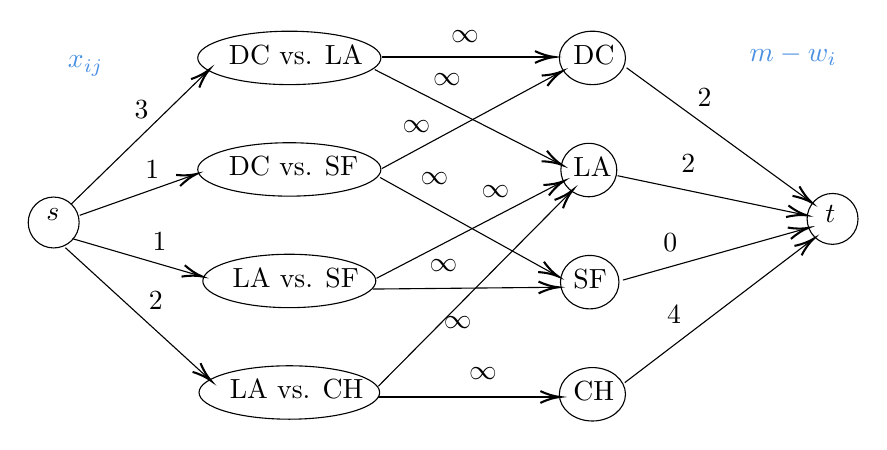
\begin{tikzpicture}[x=0.65pt,y=0.65pt,yscale=-1,xscale=1]
%uncomment if require: \path (0,363); %set diagram left start at 0, and has height of 363

%Straight Lines [id:da29828191190457176] 
\draw    (96,193) -- (171.57,119.4) ;
\draw [shift={(173,118)}, rotate = 135.75] [color={rgb, 255:red, 0; green, 0; blue, 0 }  ][line width=0.75]    (10.93,-3.29) .. controls (6.95,-1.4) and (3.31,-0.3) .. (0,0) .. controls (3.31,0.3) and (6.95,1.4) .. (10.93,3.29)   ;
%Straight Lines [id:da9886659900165116] 
\draw    (101,199) -- (164.11,176.67) ;
\draw [shift={(166,176)}, rotate = 160.51] [color={rgb, 255:red, 0; green, 0; blue, 0 }  ][line width=0.75]    (10.93,-3.29) .. controls (6.95,-1.4) and (3.31,-0.3) .. (0,0) .. controls (3.31,0.3) and (6.95,1.4) .. (10.93,3.29)   ;
%Straight Lines [id:da3998356428655834] 
\draw    (97,212) -- (167.08,232.44) ;
\draw [shift={(169,233)}, rotate = 196.26] [color={rgb, 255:red, 0; green, 0; blue, 0 }  ][line width=0.75]    (10.93,-3.29) .. controls (6.95,-1.4) and (3.31,-0.3) .. (0,0) .. controls (3.31,0.3) and (6.95,1.4) .. (10.93,3.29)   ;
%Straight Lines [id:da6630478389251291] 
\draw    (93,217) -- (172.52,289.65) ;
\draw [shift={(174,291)}, rotate = 222.41] [color={rgb, 255:red, 0; green, 0; blue, 0 }  ][line width=0.75]    (10.93,-3.29) .. controls (6.95,-1.4) and (3.31,-0.3) .. (0,0) .. controls (3.31,0.3) and (6.95,1.4) .. (10.93,3.29)   ;
%Straight Lines [id:da7357950429050455] 
\draw    (269,111) -- (363,111) ;
\draw [shift={(365,111)}, rotate = 180] [color={rgb, 255:red, 0; green, 0; blue, 0 }  ][line width=0.75]    (10.93,-3.29) .. controls (6.95,-1.4) and (3.31,-0.3) .. (0,0) .. controls (3.31,0.3) and (6.95,1.4) .. (10.93,3.29)   ;
%Straight Lines [id:da20538179275924828] 
\draw    (265,118) -- (367.22,170.09) ;
\draw [shift={(369,171)}, rotate = 207] [color={rgb, 255:red, 0; green, 0; blue, 0 }  ][line width=0.75]    (10.93,-3.29) .. controls (6.95,-1.4) and (3.31,-0.3) .. (0,0) .. controls (3.31,0.3) and (6.95,1.4) .. (10.93,3.29)   ;
%Straight Lines [id:da5590976987316391] 
\draw    (269,173) -- (367.24,119.95) ;
\draw [shift={(369,119)}, rotate = 151.63] [color={rgb, 255:red, 0; green, 0; blue, 0 }  ][line width=0.75]    (10.93,-3.29) .. controls (6.95,-1.4) and (3.31,-0.3) .. (0,0) .. controls (3.31,0.3) and (6.95,1.4) .. (10.93,3.29)   ;
%Straight Lines [id:da12638756166282472] 
\draw    (268,178) -- (365.25,232.03) ;
\draw [shift={(367,233)}, rotate = 209.05] [color={rgb, 255:red, 0; green, 0; blue, 0 }  ][line width=0.75]    (10.93,-3.29) .. controls (6.95,-1.4) and (3.31,-0.3) .. (0,0) .. controls (3.31,0.3) and (6.95,1.4) .. (10.93,3.29)   ;
%Straight Lines [id:da5033534492664359] 
\draw    (266,234) -- (368.23,180.92) ;
\draw [shift={(370,180)}, rotate = 152.56] [color={rgb, 255:red, 0; green, 0; blue, 0 }  ][line width=0.75]    (10.93,-3.29) .. controls (6.95,-1.4) and (3.31,-0.3) .. (0,0) .. controls (3.31,0.3) and (6.95,1.4) .. (10.93,3.29)   ;
%Straight Lines [id:da8320023848041241] 
\draw    (264,240) -- (365,239.02) ;
\draw [shift={(367,239)}, rotate = 179.44] [color={rgb, 255:red, 0; green, 0; blue, 0 }  ][line width=0.75]    (10.93,-3.29) .. controls (6.95,-1.4) and (3.31,-0.3) .. (0,0) .. controls (3.31,0.3) and (6.95,1.4) .. (10.93,3.29)   ;
%Straight Lines [id:da12872737382850508] 
\draw    (267,294) -- (373.59,186.42) ;
\draw [shift={(375,185)}, rotate = 134.74] [color={rgb, 255:red, 0; green, 0; blue, 0 }  ][line width=0.75]    (10.93,-3.29) .. controls (6.95,-1.4) and (3.31,-0.3) .. (0,0) .. controls (3.31,0.3) and (6.95,1.4) .. (10.93,3.29)   ;
%Straight Lines [id:da8484636178289252] 
\draw    (267,300) -- (366,300) ;
\draw [shift={(368,300)}, rotate = 180] [color={rgb, 255:red, 0; green, 0; blue, 0 }  ][line width=0.75]    (10.93,-3.29) .. controls (6.95,-1.4) and (3.31,-0.3) .. (0,0) .. controls (3.31,0.3) and (6.95,1.4) .. (10.93,3.29)   ;
%Straight Lines [id:da0981113218239027] 
\draw    (404,292) -- (507.41,213.21) ;
\draw [shift={(509,212)}, rotate = 142.7] [color={rgb, 255:red, 0; green, 0; blue, 0 }  ][line width=0.75]    (10.93,-3.29) .. controls (6.95,-1.4) and (3.31,-0.3) .. (0,0) .. controls (3.31,0.3) and (6.95,1.4) .. (10.93,3.29)   ;
%Straight Lines [id:da7431038981588827] 
\draw    (403,235) -- (504.07,206.54) ;
\draw [shift={(506,206)}, rotate = 164.28] [color={rgb, 255:red, 0; green, 0; blue, 0 }  ][line width=0.75]    (10.93,-3.29) .. controls (6.95,-1.4) and (3.31,-0.3) .. (0,0) .. controls (3.31,0.3) and (6.95,1.4) .. (10.93,3.29)   ;
%Straight Lines [id:da46241455607409654] 
\draw    (400,177) -- (503.04,198.59) ;
\draw [shift={(505,199)}, rotate = 191.83] [color={rgb, 255:red, 0; green, 0; blue, 0 }  ][line width=0.75]    (10.93,-3.29) .. controls (6.95,-1.4) and (3.31,-0.3) .. (0,0) .. controls (3.31,0.3) and (6.95,1.4) .. (10.93,3.29)   ;
%Straight Lines [id:da29204844875012814] 
\draw    (405,117) -- (506.38,190.82) ;
\draw [shift={(508,192)}, rotate = 216.06] [color={rgb, 255:red, 0; green, 0; blue, 0 }  ][line width=0.75]    (10.93,-3.29) .. controls (6.95,-1.4) and (3.31,-0.3) .. (0,0) .. controls (3.31,0.3) and (6.95,1.4) .. (10.93,3.29)   ;

% Text Node
\draw    (217.5, 111.5) circle [x radius= 50.91, y radius= 14.85]   ;
\draw (182.5,103) node [anchor=north west][inner sep=0.75pt]   [align=left] {DC vs. LA};
% Text Node
\draw    (217.5, 173.5) circle [x radius= 50.91, y radius= 14.85]   ;
\draw (182.5,165) node [anchor=north west][inner sep=0.75pt]   [align=left] {DC vs. SF};
% Text Node
\draw    (217.5, 235.5) circle [x radius= 48.08, y radius= 14.85]   ;
\draw (184.5,227) node [anchor=north west][inner sep=0.75pt]   [align=left] {LA vs. SF};
% Text Node
\draw    (217.5, 297.5) circle [x radius= 50.2, y radius= 14.85]   ;
\draw (183,289) node [anchor=north west][inner sep=0.75pt]   [align=left] {LA vs. CH};
% Text Node
\draw    (86.5, 203) circle [x radius= 14.15, y radius= 14.15]   ;
\draw (81,194) node [anchor=north west][inner sep=0.75pt]   [align=left] {$\displaystyle s$};
% Text Node
\draw    (386, 111.5) circle [x radius= 18.38, y radius= 14.85]   ;
\draw (374,103) node [anchor=north west][inner sep=0.75pt]   [align=left] {DC};
% Text Node
\draw    (384, 173.83) circle [x radius= 15.56, y radius= 14.85]   ;
\draw (374,165.33) node [anchor=north west][inner sep=0.75pt]   [align=left] {LA};
% Text Node
\draw    (384.5, 236.16) circle [x radius= 16.26, y radius= 14.85]   ;
\draw (374,227.66) node [anchor=north west][inner sep=0.75pt]   [align=left] {SF};
% Text Node
\draw    (386, 298.5) circle [x radius= 18.38, y radius= 14.85]   ;
\draw (374,290) node [anchor=north west][inner sep=0.75pt]   [align=left] {CH};
% Text Node
\draw    (519.5, 201) circle [x radius= 14.15, y radius= 14.15]   ;
\draw (514,192) node [anchor=north west][inner sep=0.75pt]   [align=left] {$\displaystyle t$};
% Text Node
\draw (130,134) node [anchor=north west][inner sep=0.75pt]   [align=left] {3};
% Text Node
\draw (136,167) node [anchor=north west][inner sep=0.75pt]   [align=left] {1};
% Text Node
\draw (140,207) node [anchor=north west][inner sep=0.75pt]   [align=left] {1};
% Text Node
\draw (138,240) node [anchor=north west][inner sep=0.75pt]   [align=left] {2};
% Text Node
\draw (443,127) node [anchor=north west][inner sep=0.75pt]   [align=left] {2};
% Text Node
\draw (434,164) node [anchor=north west][inner sep=0.75pt]   [align=left] {2};
% Text Node
\draw (424,208) node [anchor=north west][inner sep=0.75pt]   [align=left] {0};
% Text Node
\draw (426,248) node [anchor=north west][inner sep=0.75pt]   [align=left] {4};
% Text Node
\draw (306,95) node [anchor=north west][inner sep=0.75pt]   [align=left] {$\displaystyle \infty $};
% Text Node
\draw (296,119) node [anchor=north west][inner sep=0.75pt]   [align=left] {$\displaystyle \infty $};
% Text Node
\draw (279,145) node [anchor=north west][inner sep=0.75pt]   [align=left] {$\displaystyle \infty $};
% Text Node
\draw (289,174) node [anchor=north west][inner sep=0.75pt]   [align=left] {$\displaystyle \infty $};
% Text Node
\draw (323,181) node [anchor=north west][inner sep=0.75pt]   [align=left] {$\displaystyle \infty $};
% Text Node
\draw (294,222) node [anchor=north west][inner sep=0.75pt]   [align=left] {$\displaystyle \infty $};
% Text Node
\draw (302,254) node [anchor=north west][inner sep=0.75pt]   [align=left] {$\displaystyle \infty $};
% Text Node
\draw (316,282) node [anchor=north west][inner sep=0.75pt]   [align=left] {$\displaystyle \infty $};
% Text Node
\draw (93,109) node [anchor=north west][inner sep=0.75pt]  [color={rgb, 255:red, 74; green, 144; blue, 226 }  ,opacity=1 ] [align=left] {$\displaystyle x_{ij}$};
% Text Node
\draw (472,103) node [anchor=north west][inner sep=0.75pt]  [color={rgb, 255:red, 74; green, 144; blue, 226 }  ,opacity=1 ] [align=left] {$\displaystyle m-w_{i}$};


\end{tikzpicture}

}
\caption{The network constructed from the instance given above.}
\label{fig:baseball}
\end{figure}

Next, the algorithm computes an maximum flow $f^*$.
The algorithm returns true~(i.e., $T_1$ can still win the first place)
if $|f^*| = \sum_{2\le i< j \le n} x_{ij}$, i.e., all future wins
\emph{can} be distributed while guaranteeing that $T_i$ receive no 
more than $m-w_i$ wins for all $2\le i \le n$. Note that
in this case, such a distribution~(i.e., outcomes of future games)
is given by $f^*$. The algorithm returns false~(i.e., $T_1$ is already out
regardless the outcome of future games) if $|f^*| < \sum_{2\le i< j \le n} x_{ij}$.

The correctness of above algorithm follows an argument that,
there exists a one-to-one correspondence beween
an outcome of all future games~(i.e., an assignment of all wins to teams)
that gives no more than $m-w_i$ additional wins to $T_i$
and a flow $f$ with $|f| = \sum_{2\le i < j \le n} x_{ij}$.
Since the algorithm decides the latter, it answers the former correctly.



In the case of $|f^*| < \sum_{2\le i< j \le n} x_{ij}$,
a certificate can be constructed, by computing an minimum $s$-$t$ cut $(S^*, T^*)$,
and collect the teams in $S^*$ as the certificate $C$.
See Figure~\ref{fig:certificate}.
We now prove this is correct, by starting with characterizing
the structure of this minimum $s$-$t$ cut $(S^*,T^*)$.

\begin{figure}[!h]
\centering{

\tikzset{every picture/.style={line width=0.75pt}} %set default line width to 0.75pt        

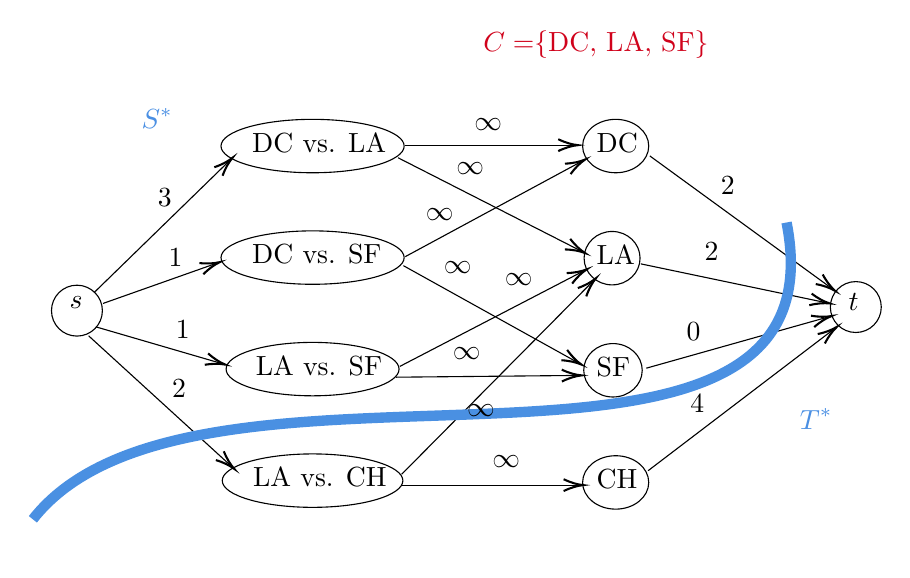
\begin{tikzpicture}[x=0.65pt,y=0.65pt,yscale=-1,xscale=1]
%uncomment if require: \path (0,459); %set diagram left start at 0, and has height of 459

%Straight Lines [id:da29828191190457176] 
\draw    (95,153) -- (170.57,79.4) ;
\draw [shift={(172,78)}, rotate = 135.75] [color={rgb, 255:red, 0; green, 0; blue, 0 }  ][line width=0.75]    (10.93,-3.29) .. controls (6.95,-1.4) and (3.31,-0.3) .. (0,0) .. controls (3.31,0.3) and (6.95,1.4) .. (10.93,3.29)   ;
%Straight Lines [id:da9886659900165116] 
\draw    (100,159) -- (163.11,136.67) ;
\draw [shift={(165,136)}, rotate = 160.51] [color={rgb, 255:red, 0; green, 0; blue, 0 }  ][line width=0.75]    (10.93,-3.29) .. controls (6.95,-1.4) and (3.31,-0.3) .. (0,0) .. controls (3.31,0.3) and (6.95,1.4) .. (10.93,3.29)   ;
%Straight Lines [id:da3998356428655834] 
\draw    (96,172) -- (166.08,192.44) ;
\draw [shift={(168,193)}, rotate = 196.26] [color={rgb, 255:red, 0; green, 0; blue, 0 }  ][line width=0.75]    (10.93,-3.29) .. controls (6.95,-1.4) and (3.31,-0.3) .. (0,0) .. controls (3.31,0.3) and (6.95,1.4) .. (10.93,3.29)   ;
%Straight Lines [id:da6630478389251291] 
\draw    (92,177) -- (171.52,249.65) ;
\draw [shift={(173,251)}, rotate = 222.41] [color={rgb, 255:red, 0; green, 0; blue, 0 }  ][line width=0.75]    (10.93,-3.29) .. controls (6.95,-1.4) and (3.31,-0.3) .. (0,0) .. controls (3.31,0.3) and (6.95,1.4) .. (10.93,3.29)   ;
%Straight Lines [id:da7357950429050455] 
\draw    (268,71) -- (362,71) ;
\draw [shift={(364,71)}, rotate = 180] [color={rgb, 255:red, 0; green, 0; blue, 0 }  ][line width=0.75]    (10.93,-3.29) .. controls (6.95,-1.4) and (3.31,-0.3) .. (0,0) .. controls (3.31,0.3) and (6.95,1.4) .. (10.93,3.29)   ;
%Straight Lines [id:da20538179275924828] 
\draw    (264,78) -- (366.22,130.09) ;
\draw [shift={(368,131)}, rotate = 207] [color={rgb, 255:red, 0; green, 0; blue, 0 }  ][line width=0.75]    (10.93,-3.29) .. controls (6.95,-1.4) and (3.31,-0.3) .. (0,0) .. controls (3.31,0.3) and (6.95,1.4) .. (10.93,3.29)   ;
%Straight Lines [id:da5590976987316391] 
\draw    (268,133) -- (366.24,79.95) ;
\draw [shift={(368,79)}, rotate = 151.63] [color={rgb, 255:red, 0; green, 0; blue, 0 }  ][line width=0.75]    (10.93,-3.29) .. controls (6.95,-1.4) and (3.31,-0.3) .. (0,0) .. controls (3.31,0.3) and (6.95,1.4) .. (10.93,3.29)   ;
%Straight Lines [id:da12638756166282472] 
\draw    (267,138) -- (364.25,192.03) ;
\draw [shift={(366,193)}, rotate = 209.05] [color={rgb, 255:red, 0; green, 0; blue, 0 }  ][line width=0.75]    (10.93,-3.29) .. controls (6.95,-1.4) and (3.31,-0.3) .. (0,0) .. controls (3.31,0.3) and (6.95,1.4) .. (10.93,3.29)   ;
%Straight Lines [id:da5033534492664359] 
\draw    (265,194) -- (367.23,140.92) ;
\draw [shift={(369,140)}, rotate = 152.56] [color={rgb, 255:red, 0; green, 0; blue, 0 }  ][line width=0.75]    (10.93,-3.29) .. controls (6.95,-1.4) and (3.31,-0.3) .. (0,0) .. controls (3.31,0.3) and (6.95,1.4) .. (10.93,3.29)   ;
%Straight Lines [id:da8320023848041241] 
\draw    (263,200) -- (364,199.02) ;
\draw [shift={(366,199)}, rotate = 179.44] [color={rgb, 255:red, 0; green, 0; blue, 0 }  ][line width=0.75]    (10.93,-3.29) .. controls (6.95,-1.4) and (3.31,-0.3) .. (0,0) .. controls (3.31,0.3) and (6.95,1.4) .. (10.93,3.29)   ;
%Straight Lines [id:da12872737382850508] 
\draw    (266,254) -- (372.59,146.42) ;
\draw [shift={(374,145)}, rotate = 134.74] [color={rgb, 255:red, 0; green, 0; blue, 0 }  ][line width=0.75]    (10.93,-3.29) .. controls (6.95,-1.4) and (3.31,-0.3) .. (0,0) .. controls (3.31,0.3) and (6.95,1.4) .. (10.93,3.29)   ;
%Straight Lines [id:da8484636178289252] 
\draw    (266,260) -- (365,260) ;
\draw [shift={(367,260)}, rotate = 180] [color={rgb, 255:red, 0; green, 0; blue, 0 }  ][line width=0.75]    (10.93,-3.29) .. controls (6.95,-1.4) and (3.31,-0.3) .. (0,0) .. controls (3.31,0.3) and (6.95,1.4) .. (10.93,3.29)   ;
%Straight Lines [id:da0981113218239027] 
\draw    (403,252) -- (506.41,173.21) ;
\draw [shift={(508,172)}, rotate = 142.7] [color={rgb, 255:red, 0; green, 0; blue, 0 }  ][line width=0.75]    (10.93,-3.29) .. controls (6.95,-1.4) and (3.31,-0.3) .. (0,0) .. controls (3.31,0.3) and (6.95,1.4) .. (10.93,3.29)   ;
%Straight Lines [id:da7431038981588827] 
\draw    (402,195) -- (503.07,166.54) ;
\draw [shift={(505,166)}, rotate = 164.28] [color={rgb, 255:red, 0; green, 0; blue, 0 }  ][line width=0.75]    (10.93,-3.29) .. controls (6.95,-1.4) and (3.31,-0.3) .. (0,0) .. controls (3.31,0.3) and (6.95,1.4) .. (10.93,3.29)   ;
%Straight Lines [id:da46241455607409654] 
\draw    (399,137) -- (502.04,158.59) ;
\draw [shift={(504,159)}, rotate = 191.83] [color={rgb, 255:red, 0; green, 0; blue, 0 }  ][line width=0.75]    (10.93,-3.29) .. controls (6.95,-1.4) and (3.31,-0.3) .. (0,0) .. controls (3.31,0.3) and (6.95,1.4) .. (10.93,3.29)   ;
%Straight Lines [id:da29204844875012814] 
\draw    (404,77) -- (505.38,150.82) ;
\draw [shift={(507,152)}, rotate = 216.06] [color={rgb, 255:red, 0; green, 0; blue, 0 }  ][line width=0.75]    (10.93,-3.29) .. controls (6.95,-1.4) and (3.31,-0.3) .. (0,0) .. controls (3.31,0.3) and (6.95,1.4) .. (10.93,3.29)   ;
%Curve Lines [id:da09781064377979187] 
\draw [color={rgb, 255:red, 74; green, 144; blue, 226 }  ,draw opacity=1 ][line width=3.75]    (61,279) .. controls (152,163) and (515,293) .. (480,114) ;

% Text Node
\draw    (216.5, 71.5) circle [x radius= 50.91, y radius= 14.85]   ;
\draw (181.5,63) node [anchor=north west][inner sep=0.75pt]   [align=left] {DC vs. LA};
% Text Node
\draw    (216.5, 133.5) circle [x radius= 50.91, y radius= 14.85]   ;
\draw (181.5,125) node [anchor=north west][inner sep=0.75pt]   [align=left] {DC vs. SF};
% Text Node
\draw    (216.5, 195.5) circle [x radius= 48.08, y radius= 14.85]   ;
\draw (183.5,187) node [anchor=north west][inner sep=0.75pt]   [align=left] {LA vs. SF};
% Text Node
\draw    (216.5, 257.5) circle [x radius= 50.2, y radius= 14.85]   ;
\draw (182,249) node [anchor=north west][inner sep=0.75pt]   [align=left] {LA vs. CH};
% Text Node
\draw    (85.5, 163) circle [x radius= 14.15, y radius= 14.15]   ;
\draw (80,154) node [anchor=north west][inner sep=0.75pt]   [align=left] {$\displaystyle s$};
% Text Node
\draw    (385, 71.5) circle [x radius= 18.38, y radius= 14.85]   ;
\draw (373,63) node [anchor=north west][inner sep=0.75pt]   [align=left] {DC};
% Text Node
\draw    (383, 133.83) circle [x radius= 15.56, y radius= 14.85]   ;
\draw (373,125.33) node [anchor=north west][inner sep=0.75pt]   [align=left] {LA};
% Text Node
\draw    (383.5, 196.16) circle [x radius= 16.26, y radius= 14.85]   ;
\draw (373,187.66) node [anchor=north west][inner sep=0.75pt]   [align=left] {SF};
% Text Node
\draw    (385, 258.5) circle [x radius= 18.38, y radius= 14.85]   ;
\draw (373,250) node [anchor=north west][inner sep=0.75pt]   [align=left] {CH};
% Text Node
\draw    (518.5, 161) circle [x radius= 14.15, y radius= 14.15]   ;
\draw (513,152) node [anchor=north west][inner sep=0.75pt]   [align=left] {$\displaystyle t$};
% Text Node
\draw (129,94) node [anchor=north west][inner sep=0.75pt]   [align=left] {3};
% Text Node
\draw (135,127) node [anchor=north west][inner sep=0.75pt]   [align=left] {1};
% Text Node
\draw (139,167) node [anchor=north west][inner sep=0.75pt]   [align=left] {1};
% Text Node
\draw (137,200) node [anchor=north west][inner sep=0.75pt]   [align=left] {2};
% Text Node
\draw (442,87) node [anchor=north west][inner sep=0.75pt]   [align=left] {2};
% Text Node
\draw (433,124) node [anchor=north west][inner sep=0.75pt]   [align=left] {2};
% Text Node
\draw (423,168) node [anchor=north west][inner sep=0.75pt]   [align=left] {0};
% Text Node
\draw (425,208) node [anchor=north west][inner sep=0.75pt]   [align=left] {4};
% Text Node
\draw (305,55) node [anchor=north west][inner sep=0.75pt]   [align=left] {$\displaystyle \infty $};
% Text Node
\draw (295,79) node [anchor=north west][inner sep=0.75pt]   [align=left] {$\displaystyle \infty $};
% Text Node
\draw (278,105) node [anchor=north west][inner sep=0.75pt]   [align=left] {$\displaystyle \infty $};
% Text Node
\draw (288,134) node [anchor=north west][inner sep=0.75pt]   [align=left] {$\displaystyle \infty $};
% Text Node
\draw (322,141) node [anchor=north west][inner sep=0.75pt]   [align=left] {$\displaystyle \infty $};
% Text Node
\draw (293,182) node [anchor=north west][inner sep=0.75pt]   [align=left] {$\displaystyle \infty $};
% Text Node
\draw (301,214) node [anchor=north west][inner sep=0.75pt]   [align=left] {$\displaystyle \infty $};
% Text Node
\draw (315,242) node [anchor=north west][inner sep=0.75pt]   [align=left] {$\displaystyle \infty $};
% Text Node
\draw (310,6) node [anchor=north west][inner sep=0.75pt]  [color={rgb, 255:red, 208; green, 2; blue, 27 }  ,opacity=1 ] [align=left] {$\displaystyle C=$\{DC, LA, SF\}};
% Text Node
\draw (486,216) node [anchor=north west][inner sep=0.75pt]  [color={rgb, 255:red, 74; green, 144; blue, 226 }  ,opacity=1 ] [align=left] {$\displaystyle \textcolor[rgb]{0.29,0.56,0.89}{T^{*}}$};
% Text Node
\draw (120,49) node [anchor=north west][inner sep=0.75pt]  [color={rgb, 255:red, 74; green, 144; blue, 226 }  ,opacity=1 ] [align=left] {$\displaystyle \textcolor[rgb]{0.29,0.56,0.89}{S^{*}}$};


\end{tikzpicture}

}
\caption{Constructing a certificate $C$ showing that $T_1$ is already out,
	by computing a minimum $s$-$t$ cut $(S^*,T^*)$ and collecting the teams in $S^*$.}
\label{fig:certificate}
\end{figure}



\begin{fact}
$(T_i,T_j) \in S^*$ if and only if $T_i\in S^*$ and $T_j\in S^*$.
\label{fact:ball}
\end{fact}
\emph{Proof.} 
See Figure~\ref{fig:ballproof}.
We first prove ``$\Longrightarrow$''.
Without loss of generality, assume conversely that $T_i \not\in S^*$.
This means that the edge from $(T_i,T_j)$ to $T_i$ is a cut-edge.
Since this edge has a capacity of $\infty$, we have $c(S^*,T^*) = \infty$, a contradiction.
Now we prove ``$\Longleftarrow$''. 
Assume conversely that $(T_i, T_j)$ is in $T^*$.
Consider all edges adjacent to $(T_i, T_j)$;
the edge from $s$ to $(T_i,T_j)$ is one of the cut-edges, but not the other two edges.
Now, we move $(T_i,T_j)$ to $S^*$.
In this new $s$-$t$ cut, the edge $s$ to $(T_i,T_j)$ is not a cut-edge any more,
implying that this new cut has a smaller capacity than $(S^*,T^*)$, a contradiction.  \qed

\begin{figure}[!h]
\centering{

\tikzset{every picture/.style={line width=0.75pt}} %set default line width to 0.75pt        

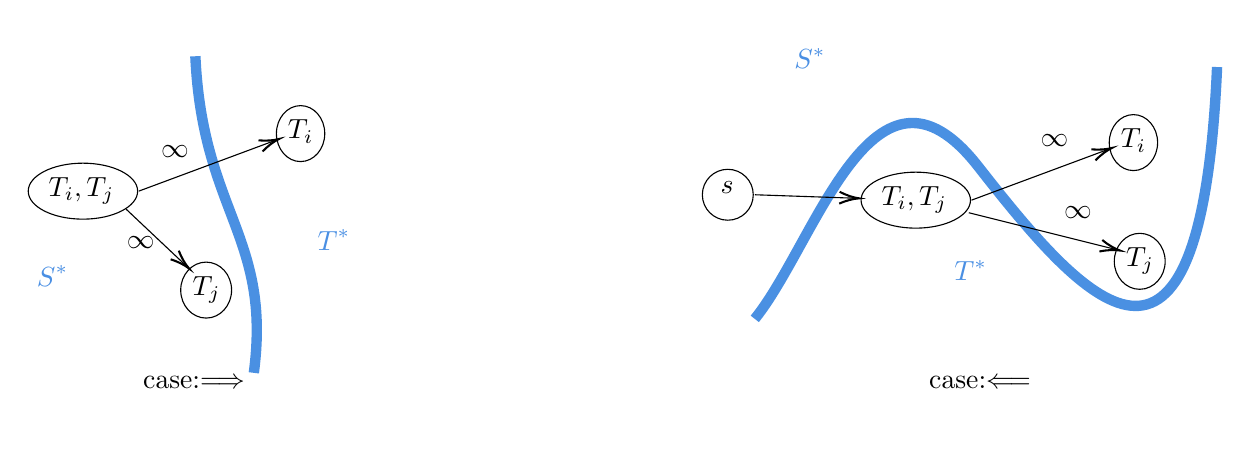
\begin{tikzpicture}[x=0.65pt,y=0.65pt,yscale=-1,xscale=1]
%uncomment if require: \path (0,459); %set diagram left start at 0, and has height of 459

%Curve Lines [id:da054999626964672865] 
\draw [color={rgb, 255:red, 74; green, 144; blue, 226 }  ,draw opacity=1 ][line width=3.75]    (166,265) .. controls (176,189) and (137.5,176) .. (133.5,89) ;
%Straight Lines [id:da2789805505394123] 
\draw    (102,164) -- (178.13,135.7) ;
\draw [shift={(180,135)}, rotate = 159.61] [color={rgb, 255:red, 0; green, 0; blue, 0 }  ][line width=0.75]    (10.93,-3.29) .. controls (6.95,-1.4) and (3.31,-0.3) .. (0,0) .. controls (3.31,0.3) and (6.95,1.4) .. (10.93,3.29)   ;
%Straight Lines [id:da48164084756462144] 
\draw    (95,174) -- (128.54,205.63) ;
\draw [shift={(130,207)}, rotate = 223.32] [color={rgb, 255:red, 0; green, 0; blue, 0 }  ][line width=0.75]    (10.93,-3.29) .. controls (6.95,-1.4) and (3.31,-0.3) .. (0,0) .. controls (3.31,0.3) and (6.95,1.4) .. (10.93,3.29)   ;
%Curve Lines [id:da16276842775686318] 
\draw [color={rgb, 255:red, 74; green, 144; blue, 226 }  ,draw opacity=1 ][line width=3.75]    (444.5,235) .. controls (478.5,193) and (510.5,76) .. (568.63,150.18) .. controls (626.75,224.35) and (692.5,301) .. (701.5,95) ;
%Straight Lines [id:da5400494970222413] 
\draw    (565,169) -- (641.13,140.7) ;
\draw [shift={(643,140)}, rotate = 159.61] [color={rgb, 255:red, 0; green, 0; blue, 0 }  ][line width=0.75]    (10.93,-3.29) .. controls (6.95,-1.4) and (3.31,-0.3) .. (0,0) .. controls (3.31,0.3) and (6.95,1.4) .. (10.93,3.29)   ;
%Straight Lines [id:da8447819866227777] 
\draw    (563.5,176) -- (645.56,196.51) ;
\draw [shift={(647.5,197)}, rotate = 194.04] [color={rgb, 255:red, 0; green, 0; blue, 0 }  ][line width=0.75]    (10.93,-3.29) .. controls (6.95,-1.4) and (3.31,-0.3) .. (0,0) .. controls (3.31,0.3) and (6.95,1.4) .. (10.93,3.29)   ;
%Straight Lines [id:da34298456292109847] 
\draw    (444.5,166) -- (500.5,167.93) ;
\draw [shift={(502.5,168)}, rotate = 181.97] [color={rgb, 255:red, 0; green, 0; blue, 0 }  ][line width=0.75]    (10.93,-3.29) .. controls (6.95,-1.4) and (3.31,-0.3) .. (0,0) .. controls (3.31,0.3) and (6.95,1.4) .. (10.93,3.29)   ;

% Text Node
\draw    (71, 164) circle [x radius= 30.41, y radius= 15.56]   ;
\draw (50.5,155) node [anchor=north west][inner sep=0.75pt]   [align=left] {$\displaystyle T_{i} ,T_{j}$};
% Text Node
\draw    (192, 132) circle [x radius= 13.44, y radius= 15.56]   ;
\draw (183.5,123) node [anchor=north west][inner sep=0.75pt]   [align=left] {$\displaystyle T_{i}$};
% Text Node
\draw (113,137) node [anchor=north west][inner sep=0.75pt]   [align=left] {$\displaystyle \infty $};
% Text Node
\draw    (139.5, 219) circle [x radius= 14.14, y radius= 15.56]   ;
\draw (130.5,210) node [anchor=north west][inner sep=0.75pt]   [align=left] {$\displaystyle T_{j}$};
% Text Node
\draw (94,188) node [anchor=north west][inner sep=0.75pt]   [align=left] {$\displaystyle \infty $};
% Text Node
\draw (200,184) node [anchor=north west][inner sep=0.75pt]  [color={rgb, 255:red, 74; green, 144; blue, 226 }  ,opacity=1 ] [align=left] {$\displaystyle \textcolor[rgb]{0.29,0.56,0.89}{T}\textcolor[rgb]{0.29,0.56,0.89}{^{*}}$};
% Text Node
\draw (44,204) node [anchor=north west][inner sep=0.75pt]  [color={rgb, 255:red, 74; green, 144; blue, 226 }  ,opacity=1 ] [align=left] {$\displaystyle \textcolor[rgb]{0.29,0.56,0.89}{S}\textcolor[rgb]{0.29,0.56,0.89}{^{*}}$};
% Text Node
\draw    (534, 169) circle [x radius= 30.41, y radius= 15.56]   ;
\draw (513.5,160) node [anchor=north west][inner sep=0.75pt]   [align=left] {$\displaystyle T_{i} ,T_{j}$};
% Text Node
\draw    (655, 137) circle [x radius= 13.44, y radius= 15.56]   ;
\draw (646.5,128) node [anchor=north west][inner sep=0.75pt]   [align=left] {$\displaystyle T_{i}$};
% Text Node
\draw (602,131) node [anchor=north west][inner sep=0.75pt]   [align=left] {$\displaystyle \infty $};
% Text Node
\draw    (658.5, 203) circle [x radius= 14.14, y radius= 15.56]   ;
\draw (649.5,194) node [anchor=north west][inner sep=0.75pt]   [align=left] {$\displaystyle T_{j}$};
% Text Node
\draw (615,171) node [anchor=north west][inner sep=0.75pt]   [align=left] {$\displaystyle \infty $};
% Text Node
\draw (554,201) node [anchor=north west][inner sep=0.75pt]  [color={rgb, 255:red, 74; green, 144; blue, 226 }  ,opacity=1 ] [align=left] {$\displaystyle \textcolor[rgb]{0.29,0.56,0.89}{T}\textcolor[rgb]{0.29,0.56,0.89}{^{*}}$};
% Text Node
\draw (465,83) node [anchor=north west][inner sep=0.75pt]  [color={rgb, 255:red, 74; green, 144; blue, 226 }  ,opacity=1 ] [align=left] {$\displaystyle \textcolor[rgb]{0.29,0.56,0.89}{S}\textcolor[rgb]{0.29,0.56,0.89}{^{*}}$};
% Text Node
\draw    (429.5, 166) circle [x radius= 14.15, y radius= 14.15]   ;
\draw (424,157) node [anchor=north west][inner sep=0.75pt]   [align=left] {$\displaystyle s$};
% Text Node
\draw (103,265.5) node [anchor=north west][inner sep=0.75pt]   [align=left] {case:$\displaystyle \Longrightarrow $};
% Text Node
\draw (540,265.5) node [anchor=north west][inner sep=0.75pt]   [align=left] {case:$\displaystyle \Longleftarrow $};


\end{tikzpicture}

}
\caption{Proof of Fact~\ref{fact:ball}.}
\label{fig:ballproof}
\end{figure}


Following above fact, the network can be sketched as follows in Figure~\ref{fig:ballsketch}.
Consider the cut-edges of $(S^*,T^*)$ and its capacity.
We can write
$$c(S^*,T^*) = \sum_{T_i \not\in C \textrm{ or } T_j \not\in C} x_{ij} + \sum_{T_i\in C} (m-w_i) \\
= \sum_{2\le i \le j \le n} x_{ij} - \sum_{T_i,T_j \in C} x_{ij} + \sum_{T_i\in C} (m-w_i) $$


\begin{figure}[!h]
\centering{

\tikzset{every picture/.style={line width=0.75pt}} %set default line width to 0.75pt        

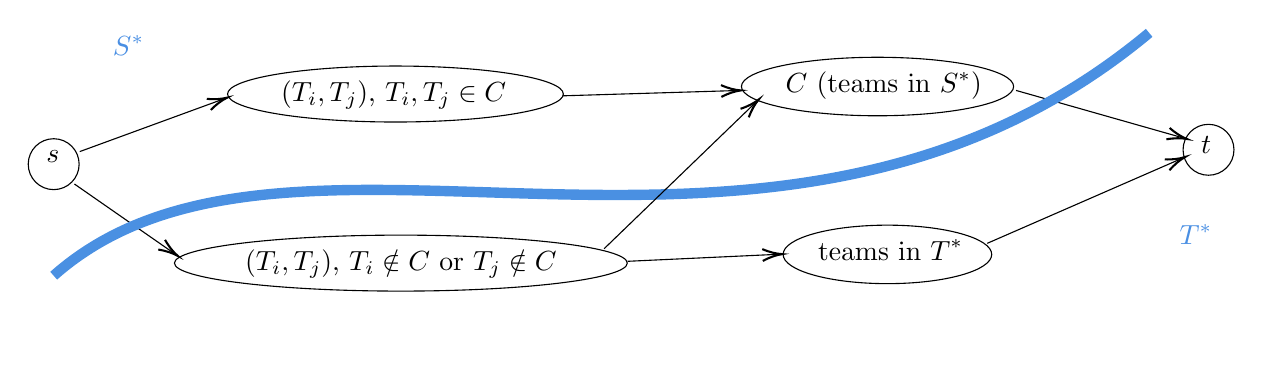
\begin{tikzpicture}[x=0.65pt,y=0.65pt,yscale=-1,xscale=1]
%uncomment if require: \path (0,264); %set diagram left start at 0, and has height of 264

%Straight Lines [id:da7772226935453113] 
\draw    (69,135) -- (149.12,105.69) ;
\draw [shift={(151,105)}, rotate = 159.9] [color={rgb, 255:red, 0; green, 0; blue, 0 }  ][line width=0.75]    (10.93,-3.29) .. controls (6.95,-1.4) and (3.31,-0.3) .. (0,0) .. controls (3.31,0.3) and (6.95,1.4) .. (10.93,3.29)   ;
%Straight Lines [id:da18617385090995575] 
\draw    (66,153) -- (121.86,191.86) ;
\draw [shift={(123.5,193)}, rotate = 214.82] [color={rgb, 255:red, 0; green, 0; blue, 0 }  ][line width=0.75]    (10.93,-3.29) .. controls (6.95,-1.4) and (3.31,-0.3) .. (0,0) .. controls (3.31,0.3) and (6.95,1.4) .. (10.93,3.29)   ;
%Straight Lines [id:da07829298607342994] 
\draw    (573.5,186) -- (681.67,138.8) ;
\draw [shift={(683.5,138)}, rotate = 156.43] [color={rgb, 255:red, 0; green, 0; blue, 0 }  ][line width=0.75]    (10.93,-3.29) .. controls (6.95,-1.4) and (3.31,-0.3) .. (0,0) .. controls (3.31,0.3) and (6.95,1.4) .. (10.93,3.29)   ;
%Straight Lines [id:da9996461500054709] 
\draw    (589.5,101) -- (682.58,127.45) ;
\draw [shift={(684.5,128)}, rotate = 195.87] [color={rgb, 255:red, 0; green, 0; blue, 0 }  ][line width=0.75]    (10.93,-3.29) .. controls (6.95,-1.4) and (3.31,-0.3) .. (0,0) .. controls (3.31,0.3) and (6.95,1.4) .. (10.93,3.29)   ;
%Curve Lines [id:da8046942013314734] 
\draw [color={rgb, 255:red, 74; green, 144; blue, 226 }  ,draw opacity=1 ][line width=3.75]    (54.5,204) .. controls (185.5,88) and (453.5,244) .. (663.5,69) ;
%Straight Lines [id:da7530738110487928] 
\draw    (337.5,104) -- (434.5,101.06) ;
\draw [shift={(436.5,101)}, rotate = 178.26] [color={rgb, 255:red, 0; green, 0; blue, 0 }  ][line width=0.75]    (10.93,-3.29) .. controls (6.95,-1.4) and (3.31,-0.3) .. (0,0) .. controls (3.31,0.3) and (6.95,1.4) .. (10.93,3.29)   ;
%Straight Lines [id:da8123228251562347] 
\draw    (373.5,196) -- (457.5,192.09) ;
\draw [shift={(459.5,192)}, rotate = 177.34] [color={rgb, 255:red, 0; green, 0; blue, 0 }  ][line width=0.75]    (10.93,-3.29) .. controls (6.95,-1.4) and (3.31,-0.3) .. (0,0) .. controls (3.31,0.3) and (6.95,1.4) .. (10.93,3.29)   ;
%Straight Lines [id:da8567126902854119] 
\draw    (360.5,189) -- (445.06,107.39) ;
\draw [shift={(446.5,106)}, rotate = 136.02] [color={rgb, 255:red, 0; green, 0; blue, 0 }  ][line width=0.75]    (10.93,-3.29) .. controls (6.95,-1.4) and (3.31,-0.3) .. (0,0) .. controls (3.31,0.3) and (6.95,1.4) .. (10.93,3.29)   ;

% Text Node
\draw    (244.5, 103) circle [x radius= 93.34, y radius= 15.56]   ;
\draw (179.5,94) node [anchor=north west][inner sep=0.75pt]   [align=left] {$\displaystyle ( T_{i} ,T_{j})$, $\displaystyle T_{i} ,T_{j} \in C$};
% Text Node
\draw    (54.5, 142) circle [x radius= 14.15, y radius= 14.15]   ;
\draw (49,133) node [anchor=north west][inner sep=0.75pt]   [align=left] {$\displaystyle s$};
% Text Node
\draw    (512.5, 98.83) circle [x radius= 75.66, y radius= 16.26]   ;
\draw (460,89.33) node [anchor=north west][inner sep=0.75pt]   [align=left] {$\displaystyle C$ (teams in $\displaystyle S^{*})$};
% Text Node
\draw    (518, 192.16) circle [x radius= 57.98, y radius= 16.26]   ;
\draw (478,182.66) node [anchor=north west][inner sep=0.75pt]   [align=left] {teams in $\displaystyle T^{*}$};
% Text Node
\draw    (696.5, 134) circle [x radius= 14.15, y radius= 14.15]   ;
\draw (691,125) node [anchor=north west][inner sep=0.75pt]   [align=left] {$\displaystyle t$};
% Text Node
\draw (679,174) node [anchor=north west][inner sep=0.75pt]  [color={rgb, 255:red, 74; green, 144; blue, 226 }  ,opacity=1 ] [align=left] {$\displaystyle \textcolor[rgb]{0.29,0.56,0.89}{T}\textcolor[rgb]{0.29,0.56,0.89}{^{*}}$};
% Text Node
\draw (86,69) node [anchor=north west][inner sep=0.75pt]  [color={rgb, 255:red, 74; green, 144; blue, 226 }  ,opacity=1 ] [align=left] {$\displaystyle \textcolor[rgb]{0.29,0.56,0.89}{S}\textcolor[rgb]{0.29,0.56,0.89}{^{*}}$};
% Text Node
\draw    (247.5, 197) circle [x radius= 125.87, y radius= 15.56]   ;
\draw (159.5,188) node [anchor=north west][inner sep=0.75pt]   [align=left] {$\displaystyle ( T_{i} ,T_{j})$, $\displaystyle T_{i} \notin C$ or $\displaystyle T_{j} \notin C$};


\end{tikzpicture}

}
\caption{Sketch of the network.}
\label{fig:ballsketch}
\end{figure}


Consider the case that $T_1$ is eliminated, i.e., $|f^*| < \sum_{2\le i< j \le n} x_{ij}$. 
Using $|f^*| = c(S^*,T^*)$, we can have that
$\sum_{T_i,T_j \in C} x_{ij} > \sum_{T_i\in C} (m-w_i)$, proving that $C$ is a certificate.

